\section{Security}
This chapter describes the considerations and decisions taken to secure the back-end application from abuse.

\subsection{Authentication}
To make sure that malicious users cannot abuse the back-end application, it was decided to secure it through authentication. 
There were two common options for how this could be handled. 

\subsubsection{The common approach}
This approach is to add a token of sorts to the header of the \gls{http} request. 
The downside of this is the missing transparency of the \gls{api}.
Headers are not immediately shown in the requests payloads and can hide the fact that authentication is necessary.
Another downside is that the interactive \gls{api} explorer \glsi{graphiql} does not support setting \gls{http} headers.

\subsubsection{The Facebook approach}
Facebook, Inc uses a root type called a \verb+viewer+ \citep{facebook:viewer}. 
The \verb+viewer+ represent the user making the request and it can be used for several things. 
What we did was to add a parameter on the root type \verb+viewer+ so that the \verb+viewer+ takes a token. 
This approach makes it very obvious that the \verb+viewer+ 'area' is restricted and requires an authentication token to access. 
Every resource that requires an authenticated user will then be underneath the \verb+viewer+ type and every other resource are exposed outside the \verb+viewer+ object. 
On figure \ref{fig:queryViewer} this is illustrated.

\graphic{0.6}{query}{\gls{api} documentation for the root query with the viewer and login queries returning the viewer type}{fig:queryViewer}

Notice that both of them return a \verb+viewer+ type. 
When logging in, the same \verb+viewer+ as you can get when asking for the \verb+viewer+ with your token, is returned. 
This is to save a round-trip after logging on, figure \ref{fig:loginSequence2}. 
Another approach is to login and only receive a token which can then be use to query for the \verb+viewer+. 
But that approach is slower as it requires two round-trips as shown on figure \ref{fig:loginSequence1}.

\begin{figure}
    \centering
    \begin{subfigure}[b]{0.45\textwidth}
        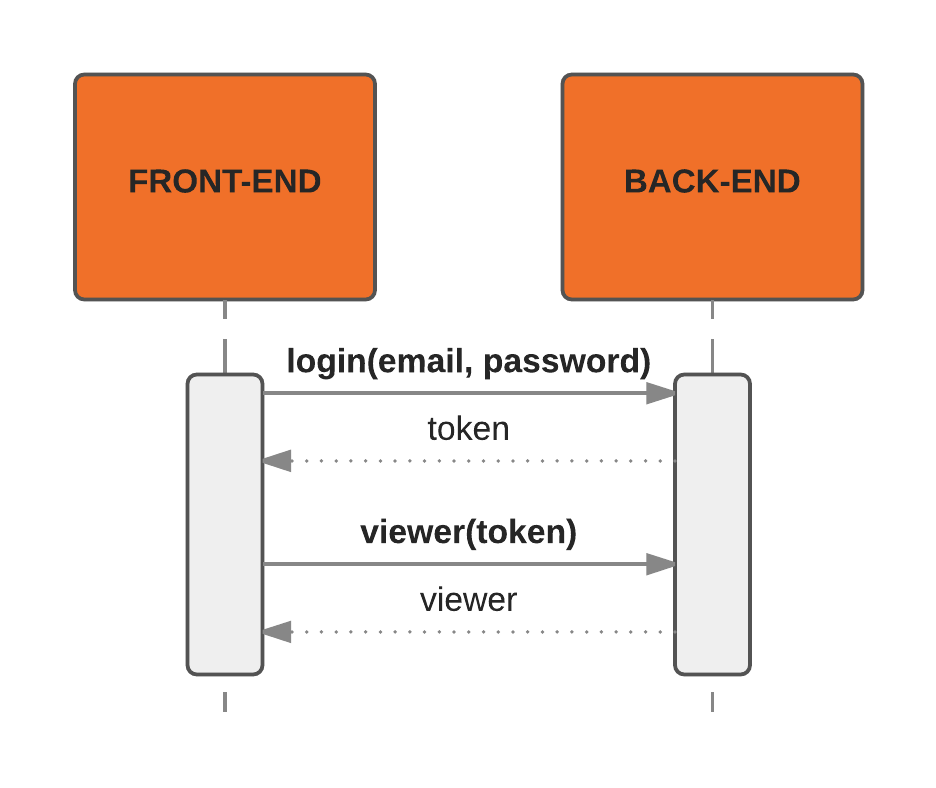
\includegraphics[width=\textwidth]{graphics/loginSequence1}
        \caption{Login returns token to further query with}
        \label{fig:loginSequence1}
    \end{subfigure}
    \hfill
    \begin{subfigure}[b]{0.45\textwidth}
        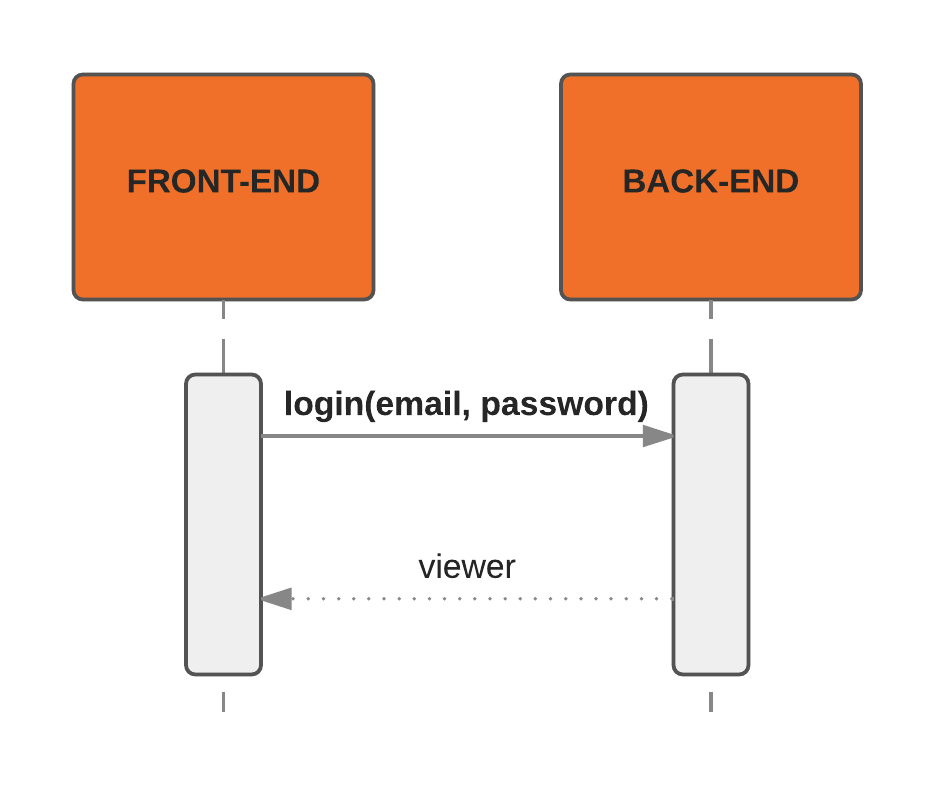
\includegraphics[width=\textwidth]{graphics/loginSequence2}
        \caption{Login returns viewer for direct access}
        \label{fig:loginSequence2}
    \end{subfigure}
    \caption{Authentication token request flows}
\end{figure}

The most important resources to get behind authentication are the mutations since they are the resources that can manipulate data. 
Because of this, all mutations are hidden behind a \verb+MutationViewer+, as shown on figure \ref{fig:mutationViewer}. 
When passing the token to the \verb+viewer+, it is checked in the database and the user owning the token, if any, is then passed down the graph so that the resources below the \verb+viewer+ knows exactly who the user is. 

\graphic{0.6}{mutation}{\gls{api} documentation for the MutationViewer type}{fig:mutationViewer}

\subsubsection{Token generation}
The token is generated on login and removed on logout. 
An \glsi{npm} package named \verb+node-uuid+ is used to generate an RFC4122 v4 \gls{uuid}, which is then stored with the user. 

The odds of creating duplicate tokens when using RFC4122 v4 is extremely small. 
On average it would take a few trillions of \gls{uuid}s to generate two duplicate tokens \citep{authentication:uuid}.
